\documentclass[submit]{harvardml}

% FDV: Update front matter -- years, dates, references to book sections, etc.
\course{CS181-S22}
\assignment{Assignment \#5}
\duedate{11:59pm EST, April 8, 2021}

\newcommand{\attr}[1]{\textsf{#1}}
\usepackage[OT1]{fontenc}
\usepackage[colorlinks,citecolor=blue,urlcolor=blue]{hyperref}
\usepackage[pdftex]{graphicx}
\usepackage{subfig}
\usepackage{framed}
\usepackage{fullpage}
\usepackage{amsmath}
\usepackage{amssymb}
\usepackage{color}
\usepackage{todonotes}
\usepackage{listings}
\usepackage{common}
\usepackage{bm}
\usepackage{enumitem}
\usepackage{tikz}
\usetikzlibrary{positioning,shapes,arrows}
% \usepackage{xifthen}
\usepackage{pythonhighlight}
\usepackage{soul}

\usepackage[mmddyyyy,hhmmss]{datetime}

\definecolor{verbgray}{gray}{0.9}

\lstnewenvironment{csv}{
  \lstset{backgroundcolor=\color{verbgray},
  frame=single,
  framerule=0pt,
  basicstyle=\ttfamily,
  columns=fullflexible}}{}

\begin{document}


\begin{center}
{\Large Homework 5: EM with Mixtures, PCA, and Graphical Models}\\
\end{center}

This homework assignment will have you work with EM for mixtures, PCA,
and graphical models. We encourage you to read sections 9.4 and 8.2.5 of the course textbook.

Please type your solutions after the corresponding problems using this
\LaTeX\ template, and start each problem on a new page.

Please submit the \textbf{writeup PDF to the Gradescope assignment `HW5'}. Remember to assign pages for each question.

Please submit your \textbf{\LaTeX\ file and code files to the Gradescope assignment `HW5 - Supplemental'}. 


\newpage
\begin{problem}[Expectation-Maximization for Gamma Mixture Models, 25pts]

In this problem we will explore expectation-maximization for a Categorical-Gamma Mixture model.

Let us suppose the following generative story for an observation $x$: first one of $K$ classes is randomly selected, and then the features $x$ are sampled according to this class. If $$z \sim \operatorname{Categorical}(\btheta)$$ indicates the selected class, then $x$ is sampled according to the class or ``component'' distribution corresponding to $z$. (Here, $\btheta$ is the mixing proportion over the $K$ components: $\sum_k \theta_k = 1$ and $ \theta_k > 0$). In this problem, we assume these component distributions are gamma distributions with shared shape parameter but different rate parameters: $$x | z \sim \operatorname{Gamma}(\alpha, \beta_k).$$

In an unsupervised setting, we are only given a set of observables as our training dataset: $\mathcal D = \{x_n\}_{n=1}^N$. The EM algorithm allows us to learn the underlying generative process (the parameters $\btheta$ and $\{\beta_k\}$) despite not having the latent variables $\{z_n\}$ corresponding to our training data.

\vspace{2em}

\begin{enumerate}

  \item \textbf{Intractability of the Data Likelihood} We are
    generally interested in finding a set of parameters $\beta_k$ that
    maximizes the likelihood of the observed data: $$\log
    p(\{x_n\}^N_{n=1}; \btheta, \{\beta_k\}^K_{k = 1}).$$ Expand the data
    likelihood to include the necessary sums over observations
    $x_n$ and to marginalize out the latents
    $\boldz_n$. Why is optimizing this likelihood directly
    intractable?

\item \textbf{Complete Data Log Likelihood} The complete dataset
  $\mathcal D = \{(x_n, \boldz_n)\}_{n=1}^N$ includes latents $\boldz_n$. Write
  out the negative complete data log likelihood: $$\mcL(\btheta, \{\beta_k\}^K_{k=1}) =  -\log p(\mathcal D; \btheta, \{\beta_k\}^K_{k=1}).$$

  Apply the power trick and simplify your expression using indicator elements $z_{n
  k}$.\footnote{The ``power trick'' is used when terms in a PDF are raised to the power of indicator components of a one-hot vector.  For example, it allows us to rewrite $p(\boldz_n ;  \btheta) = \prod_k \theta_k^{z_{nk}}$.} Notice that optimizing this loss is now computationally tractable if we know $\boldz_n$.

  (Continued on next page.)

\end{enumerate}

\end{problem}

\newpage


\begin{framed}
\noindent\textbf{Problem 1} (cont.)\\
\begin{enumerate}
\item[3.] \textbf{Expectation Step} Our next step is to introduce a
  mathematical expression for $\boldq_n$, the posterior over the
  hidden component variables~$\boldz_n$ conditioned on the observed data
  $x_n$ with fixed parameters.
That is:
  \begin{align*}
    \textbf{q}_n &= \begin{bmatrix}
      p(\boldz_n =\boldC_1| x_n; \btheta, \{ \beta_k \}^K_{k=1}) \\
      \vdots \\
      p(\boldz_n =\boldC_K| x_n; \btheta, \{ \beta_k \}^K_{k=1})
    \end{bmatrix}.
  \end{align*}
  %
%
  Write down and simplify the expression for
  $\boldq_n$.  Note that because the $\boldq_n$ represents the
  posterior over the hidden categorical variables $\boldz_n$, the
  components of vector $\boldq_n$ must sum to 1.
  The main work is to find an expression for $p(\boldz_n|x_n; \btheta, \{\beta_k\}^K_{k=1})$  for any choice of $\boldz_n$; i.e., for any 1-hot encoded $\boldz_n$. With this, you can then construct the different components that make up the vector $\boldq_n$.
  
\item[4.] \textbf{Maximization Step}
Using the~$\boldq_n$ estimates from the Expectation Step, derive an update for maximizing the expected complete data log likelihood in terms of $\btheta$ and $\{ \beta_k \}^K_{k=1}$.

\begin{enumerate}
    \item Derive an expression for the expected complete data log likelihood using $\boldq_n$.
    \item Find an expression for $\btheta$ that maximizes this expected complete data log likelihood. You may find it helpful to use Lagrange multipliers in order to enforce the constraint $\sum \theta_k = 1$. Why does this optimal $\btheta$ make intuitive sense?
    \item Find an expression for $\beta_k$ that maximizes the expected complete data log likelihood.  Why does this optimal $\beta_k$  make intuitive sense?
\end{enumerate}
    
\item[5.] Suppose that this had been a classification problem. That is,
  you were provided the ``true'' components $\boldz_n$ for each
  observation $x_n$,
  and you were going to perform the classification by
  inverting the provided generative model (i.e. now you're predicting $\boldz_n$ given $x_n$). Could you reuse any of
  your derivations above to estimate the parameters of the model?
  

\item[6.] Finally, implement your solution in \texttt{p1.ipynb} and attach the final plot below.

{\bfseries You will receive no points for code not included below.}
\end{enumerate}
  
\end{framed}

% \newpage
\subsection*{Solution}

\begin{enumerate}
  \item
  The log-likelihood we are trying to maximize is
  $$\log p(\{x_n\}^N_{n=1}; \btheta, \{\beta_k\}^K_{k = 1})$$
  $$=\sum_n\log p(x_n;\btheta \{\beta_k\}^K_{k = 1})$$
  marginalizing out our latent $\mathbf{z}_n$'s we have
  $$=\sum_n\log \left[ \sum_k p(x_n,z_{n,k};\btheta,\beta_k) \right]$$
 we can simplify no further as consolidating a summation inside of a logarithm is not possible; optimizing this likelihood directly is intractable.
  
  \item 
  The complete negative data log likelihood is 
  $$\mcL(\btheta,\{\beta_k\}^K_{k=1})$$
  $$=-\log p(D; \btheta,\{\beta_k\}^K_{k=1})$$
  $$=-\log p(\{(x_n, \mathbf{z}_n)\}^K_{k=1};\btheta,\{\beta_k\}^K_{k=1})$$
  $$=-\sum_n \log p(x_n, \mathbf{z}_n; \btheta, \{\beta_k\}^K_{k=1})$$
  $$=-\sum_n \log\left[p(x_n;\mathbf{z}_n, \{\beta_k\}^K_{k=1})p(\mathbf{z}_n;\btheta)\right]$$
  $$=-\sum_n \log p(x_n;\mathbf{z}_n, \{\beta_k\}^K_{k=1}) +\log p(\mathbf{z}_n;\btheta)$$
  using the power trick this turns into
  
  $$=-\sum_n \log\left[\prod_k\mathrm{Gamma}(x_n;\alpha,\beta_k)^{z_{n,k}}\right]+\log\left[\prod_k \theta_k^{z_{n,k}}\right]$$
  $$\boxed{\mcL(\btheta,\{\beta_k\}^K_{k=1})=-\sum_n \sum_k z_{n,k}\log\mathrm{Gamma}(x_n;\alpha,\beta_k)+z_{n,k}\log\theta_k}$$


  \item 
  Each of our $q_{n,k}$ is
  $$q_{n,k}=p(\mathbf{z}_n=C_k|x_n,\btheta,\{\beta_k\}^K_{k=1})$$
  by Bayes' rule we have
  $$q_{n,k}\propto p(x_n|\mathbf{z}_n=C_k,\{\beta_k\}^K_{k=1})p(\mathbf{z}_n=C_k;\btheta)$$
  $$= \mathrm{Gamma}(x_n;\alpha,\beta_k)^{z_{n,k}}\theta_k$$
  and to get the entire vector $\mathbf{q}_n$, we must \textbf{normalize these values} such that they sum to one, i.e.
  $$\boxed{q_{n,k}=\frac{\mathrm{Gamma}(x_n;\alpha,\beta_k)^{z_{n,k}}\theta_k}{\sum_k \mathrm{Gamma}(x_n;\alpha,\beta_k)^{z_{n,k}}\theta_k}}$$
  
  \item 
    \begin{enumerate}
      \item 
      What we want to find is the following:
      $$\mathrm{E}_{\mathbf{z}_n|x_n}\left[-\mcL(\btheta,\{\beta_k\}^K_{k=1})\right]$$
      
      we have that this is equal to
      $$=\mathrm{E}_{\mathbf{z}_n|x_n}\left[\sum_n\log p(x_n;\mathbf{z}_n,\{\beta_k\}^K_{k=1})+\log p(\mathbf{z}_n;\btheta)\right]$$
      $$=\sum_n\mathrm{E}_{\mathbf{z}_n|x_n}\left[\log p(x_n;\mathbf{z}_n,\{\beta_k\}^K_{k=1})+\log p(\mathbf{z}_n;\btheta)\right]$$
      $$=\sum_n\sum_k p(\mathbf{z}_n=C_k|x_n)\left(\log p(x_n;\mathbf{z}_n=C_k,\beta_k)+\log p(\mathbf{z}_n=C_k;\btheta)\right)$$
      $$=\sum_n\sum_k q_{n,k}\left(\log p(x_n;\mathbf{z}_n=C_k,\beta_k)+\log p(\mathbf{z}_n=C_k;\btheta)\right)$$
      $$\boxed{\mathrm{E}_{\mathbf{z}_n|x_n}\left[-\mcL(\btheta,\{\beta_k\}^K_{k=1})\right]=\sum_n\sum_k q_{n,k}\left(\log\mathrm{Gamma}(x_n;\alpha,\beta_k)+\log \theta_k\right)}$$
      
      \item 
      We wish to solve for the following
      
      $$\underset{\theta}{\mathrm{argmin}}\;\mathrm{E}_{\mathbf{z}_n|x_n}\mcL(\btheta,\{\beta_k\}^K_{k=1})\quad\text{s.t.}\quad\sum_k\theta_k -1 = 0$$
      
      we can do so using a Lagrange multiplier:
      
      $$\text{L}(\btheta, \lambda) = \mathrm{E}_{\mathbf{z}_n|x_n}\mcL(\btheta,\{\beta_k\}^K_{k=1}) + \lambda\left(\sum_{j=1}^K\theta_j-1\right)$$
      $$=-\sum_{i=1}^N\sum_{j=1}^K q_{i,j}\left(\log\mathrm{Gamma}(x_i;\alpha,\beta_j)+\log \theta_j\right)+ \lambda\left(\sum_{j=1}^K\theta_j-1\right)$$
      $$= -\sum_{i=1}^N\sum_{j=1}^K q_{i,j}\left(\alpha\log\beta_j-\log\Gamma(x_i)+(\alpha-1)\log(x_i)-\beta_j x+\log \theta_j\right) + \lambda\left(\sum_{j=1}^K\theta_j-1\right) $$
      
      the gradient with respect to $\theta_k$ of the above is

      $$\nabla_{\theta_k}\text{L}(\btheta, \lambda)=-\sum_{i=1}^N\nabla_{\theta_k} q_{i,k}(\log\theta_k)+\lambda$$
      $$=-\sum_{i=1}^N\frac{q_{i,k}}{\theta_k}+\lambda$$
      $$=-\frac{N}{\theta_k}\sum_{i=1}^N q_{i,k}+\lambda$$

      and setting this to zero to solve for $\theta_k$ yields

      $$\boxed{\theta_k =-\frac{N}{\lambda}\sum_{i=1}^N q_{i,k}}$$

      now, we do the same procedure to solve for $\lambda$ by taking the following 
      gradient and setting it to zero:

      $$\nabla_{\lambda}\text{L}(\btheta, \lambda)=\sum_{j=1}^K \theta_j -1$$

      substituting the boxed equation from above we have

      $$\nabla_{\lambda}\text{L}(\btheta, \lambda)=\sum_{j=1}^K -\frac{N}{\lambda}\sum_{i=1}^N q_{i,j} -1$$
      $$=-\frac{N}{\lambda}\sum_{j=1}^K \sum_{i=1}^N q_{i,j} -1$$

      notice that $\sum_{j=1}^K \sum_{i=1}^N q_{i,j}=N$ so we have, setting to zero,
    
      $$\nabla_{\lambda}\text{L}(\btheta, \lambda) =-\frac{N^2}{\lambda}-1=0$$
      $$\implies \boxed{\lambda=-N^2} $$

      putting together our two boxed equations we have

      $$\theta_k =-\frac{N}{-N^2}\sum_{i=1}^N q_{i,k}$$
      $$\boxed{\theta_k =\frac{1}{N}\sum_{i=1}^N q_{i,k}}$$

      this optimal value for $\theta_k$ makes sense we are averaging, over the entire data set,
      the entry of $\mathbf{q_n}$ that corresponds to the category $C_k$.

      \item
    
      We wish to solve for the following
      
      $$\underset{\{\beta_k\}^K_{k=1}}{\mathrm{argmin}}\;\mathrm{E}_{\mathbf{z}_n|x_n}\mcL(\btheta,\{\beta_k\}^K_{k=1})$$
      
      we can just differentiate with respect to $\beta_k$ here to solve this:

      $$\nabla_{\beta_k}\mathrm{E}_{\mathbf{z}_n|x_n}\mcL(\btheta,\{\beta_k\}^K_{k=1}) $$
      $$=\nabla_{\beta_k}-\sum_{i=1}^N\sum_{j=1}^K q_{i,j}\left(\log\mathrm{Gamma}(x_i;\alpha,\beta_j)+\log \theta_j\right)$$
      $$=\nabla_{\beta_k} -\sum_{i=1}^N\sum_{j=1}^K q_{i,j}\left(\alpha\log\beta_j-\log\Gamma(x_i)+(\alpha-1)\log(x_i)-\beta_j x+\log \theta_j\right) $$
      $$=-\sum_{i=1}^N \nabla_{\beta_k} [q_{i,k}\alpha\log\beta_k-q_{i,k}\beta_k x_i]$$
      $$=-\sum_{i=1}^N \frac{q_{i,k}\alpha }{\beta_k} - q_{i,k}x_i$$
      $$=-\sum_{i=1}^N \frac{q_{i,k}\alpha }{\beta_k} - q_{i,k}x_i$$
      setting this to zero yields
      $$\boxed{\beta_k = \alpha\frac{\sum_{i=1}^N q_{i,k}}{\sum_{i=1}^N q_{i,k}x_i}}$$
      this answer makes intuitive sense as $\beta_k$, the rate parameter for the gamma distribution,
      is being calculated to be negatively proportional to a weighted average of the $x_n$'s, which
      could be interpreted as times between events (such that their average is the inverse of the rate). 

    \end{enumerate}
  \item 
  Yes, except that we would no longer have to average over a ``soft" definition of $\mathbf{z}_n$, which
  is how we used $\mathbf{q}_n$.
  When calculating our loss function to minimize, instead we could directly plug in the one-hot encoded
  vector $\mathbf{z}_n$
  
  
  \item 
    Plot:

    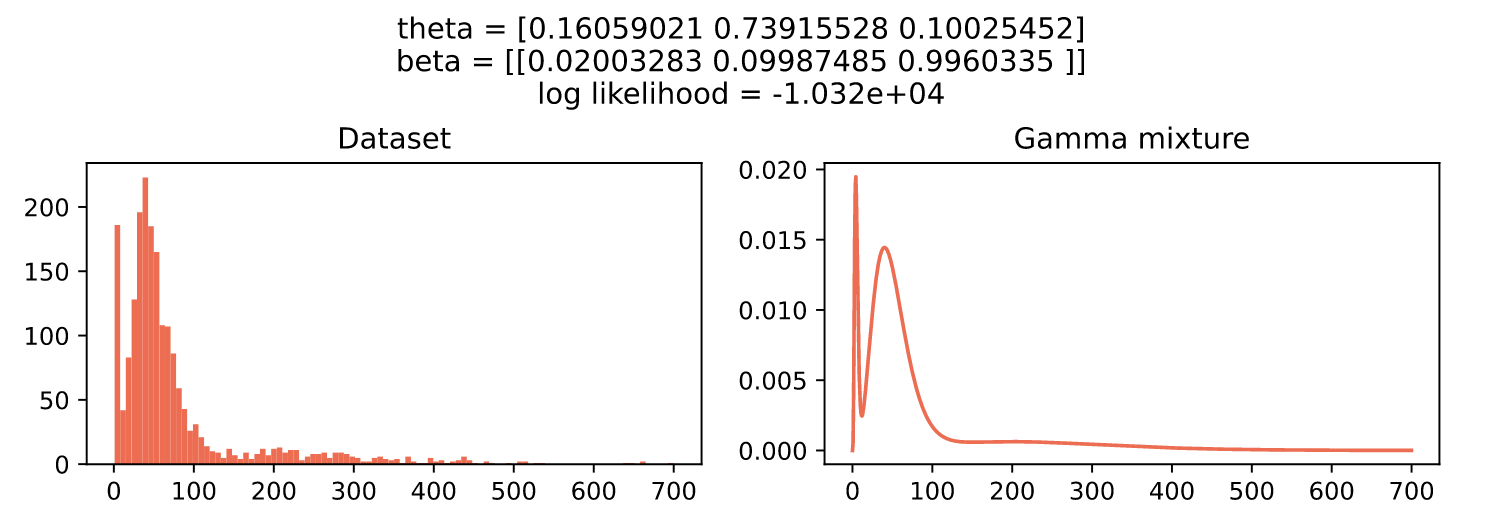
\includegraphics[width=\linewidth]{p1}

    Code:

    \begin{python}
def e_step(theta, betas):
    scales = 1 / betas
    x_given_z = gamma(alpha, scale=scales)
    q = np.multiply(x_given_z.pdf(x), theta) 
    s = np.sum(q, axis=1)
    q_normalized = np.array([q[i] / s[i] for i in range(len(q))])
    return q_normalized


def m_step(q):
    theta_hat = np.sum(q, 0) / q.shape[0]
    beta_hats = alpha * np.sum(q, 0) / (x.T @ q)
    return theta_hat, beta_hats


def log_px(x, theta, betas):
    scales = 1 / betas
    x_given_z = gamma(alpha, scale=scales)
    log_px = np.log(np.sum(np.exp(x_given_z.logpdf(x) + np.log(theta)), axis=1))
    return log_px


def run_em(theta, betas, iterations=1000):
    for _ in range(iterations):
        q = e_step(theta, betas)
        theta, betas = m_step(q)
    return theta, betas
    \end{python}
\end{enumerate}


\newpage

\begin{problem}[PCA, 15 pts]

% FDV: Here are the notes from last year.  I've already edited to make clear we want L2.  As noted below, we should also provide the baseline/reference to the pset 4 solutions in case they computed that wrong somehow.  
% 
% # problem 2 clarifications
% *NB: There was a lot of confusion about this problem, and we ended up accepting any form of comparison to PCA. Next year should clarify which norm students should use more explicitly (and maybe provide a baseline for students if the computation of the reconstruction error is different from what students calculated on pset4.)*
% 
% For Problem 2.3 (computing PCA reconstruction error), we will accept both the L1 and L2 norm and both summing over the errors for individual images and taking the mean of the errors (as long as you compute the error for K-Means the same way as you compute it for PCA). Apologies for the ambiguity in this question! 

  
For this problem you will implement PCA from scratch on the first 6000 images of the MNIST dataset. Your job is to apply PCA on MNIST and discuss what kind of structure is found. Implement your solution in \texttt{p2.ipynb} and attach the final plots below.

{\bfseries You will recieve no points for using third-party PCA implementations (i.e. {\normalfont \texttt{scikit-learn}}).}

{\bfseries You will recieve no points for code not included below.}
\begin{enumerate}

\item Compute the PCA. Plot the eigenvalues corresponding to the most
  significant 500 components in order from most significant to
  least. Make another plot that describes the cumulative proportion of
  variance explained by the first $k$ most significant components for
  values of $k$ from 1 through 500.  How much variance is explained by
  the first 500 components?  Describe how the cumulative proportion of
  variance explained changes with $k$.  Include this plot below.

\item Plot the mean image of the dataset and plot an image
  corresponding to each of the first 10 principle components.  How do
  the principle component images compare to the cluster centers from
  K-means? Discuss any similarities and differences.  Include these
  two plots below.

  \textit{Reminder: Center the data before performing PCA}

\item Compute the reconstruction error on the data set using the mean
  image of the dataset.  Then compute the reconstruction error using
  the first 10 principal components.  How do these errors compare to
  the final objective loss achieved by using K-means on the dataset?
  Discuss any similarities and differences.

  For consistency in grading, define the reconstruction error as the squared L2
  norm averaged over all data points.

\item Suppose you took the original matrix of principle components
  that you found $U$ and multiplied it by some rotation matrix $R$.
  Would that change the quality of the reconstruction error in the
  last problem?  The interpretation of the components?  Why or why
  not?
  
\end{enumerate}


\end{problem}

\newpage
\subsection*{Solution}
Plots:

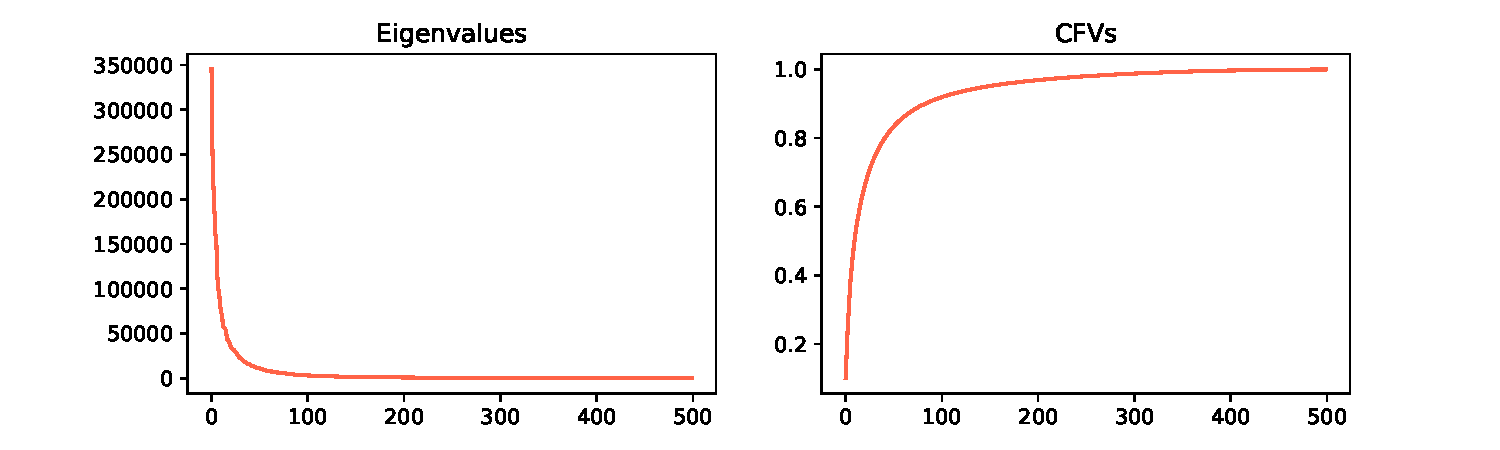
\includegraphics[width=\linewidth]{p2_cfvs}

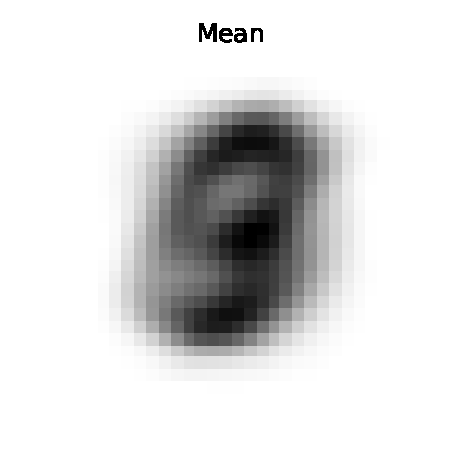
\includegraphics[width=0.25\linewidth]{p2_mean}
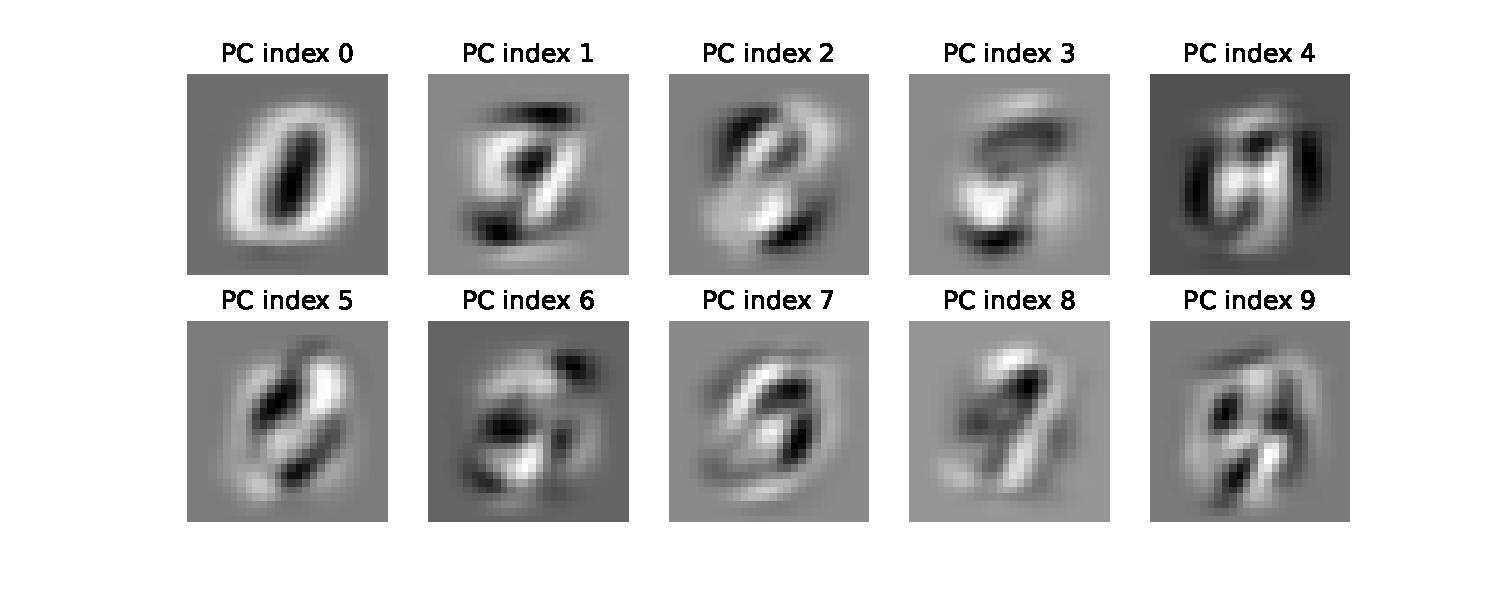
\includegraphics[width=0.75\linewidth]{p2_pcomps}

Code:

\begin{python}
def pca(x, n_comps=500):
    x = x - np.mean(x, axis=0)
    _, s, vh = np.linalg.svd(x)
    top_eigvals = s[:n_comps] ** 2 / x.shape[0]
    top_pcomps = vh[:n_comps, :]
    return top_eigvals, top_pcomps


def calc_cfvs(eigvals):
    cum_frac_vars = np.cumsum(eigvals, axis=0) / np.sum(eigvals)
    return cum_frac_vars    


def calc_errs(x, pcomps):
    x_mean = np.mean(x, axis=0)
    err_mean =np.mean(np.sum((x - x_mean) ** 2, axis=1), axis=0)
    err_pcomp = np.mean(np.sum((x - (x_mean + (x - x_mean) @ pcomps[:10, :].T @ pcomps[:10, :] )) ** 2, axis=1))
    return err_mean, err_pcomp
\end{python}

\begin{enumerate}
  \item 
  The first 500 eigenvalues of the decomposition correspond to ~0.9994 of the variance. 
  This value was calculated by running $PCA(x, n\_comps=500)$ as well as $PCA(x, n\_comps=784)$
  and calculating the sum of the former divided by the sum of the latter.
  
  \item
  I did not notice much similarity to the centers from k-means. I think this is a correct
  evaluation, as the two methods are doing something entirely different; k-means is averaging 
  images it decides are most similar, while PCA is selecting features that explain the most 
  variance. Because of this, it makes sense that k-means may somewhat resemble actual digits 
  whereas the principle components don't resemble anything like digits.
  
  \item 
  For PCA, the reconstruction error using the mean is 3.436024e+06, and the reconstruction error 
  using the 10 principle components is 1.731315e+06. The final objective loss achieved by 
  k-means on the dataset was 2.548403e+06. It makes sense that the reconstruction error
  using the mean image is the highest as it is essentially calculating the k-means objective error
  on one cluster. The reasoning behind the reconstruction error using the 10 principle components 
  being lower than the k-means objective error is more subtle--it is because k-means is simply 
  grouping close images together whereas PCA is purposefully selecting images that together
  explain the most variance in the data set.

  \item 
  This would not affect either the quality of the reconstruction error as we are
  changing the basis of the principle components which affects both dimensionality reduction
  and reconstruction equivalently, meaning it gets cancelled out in the reconstruction error 
  calculation.

  The interpretation of the components would change, however, as these would be completely changed
  relative to the data set whose variance they are trying to maximally represent.


\end{enumerate}

\newpage

\begin{problem}[Bayesian Networks, 10 pts]

% FDV: I think we can keep this problem as-is, and just clarfiy based
% on notes from last year.
% # problem 3 clarifications
% The phrasing of Q3 is slightly off because it implies that you need to explain why each path is not blocked in the case that two nodes are not independent. It is sufficient to provide a single unblocked path. Better phrasing is (emphasis added) "Use the concept of d-separation to answer the questions and show your work (i.e., state what the blocking path(s) is/are and which node blocks the path; or explain why there exists a path that is not blocked)." 
% 
% Some helpful resources for d-separation:  The 2020 Section 8 notes, Bishop p. 372 - 379, Section 8.2 of the CS 181 textbook
% 
% Problem 3: Make it clear (put the instructions in one place) that we require explanations for both "yes" and "no" answers

  
  \noindent In this problem we explore the conditional independence
  properties of a Bayesian Network.  Consider the following Bayesian
  network representing a fictitious person's activities. Each random
  variable is binary (true/false).

\begin{center}
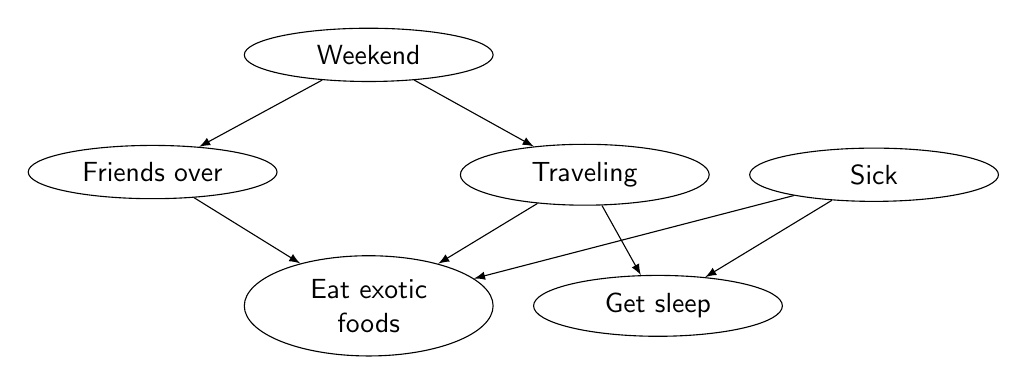
\begin{tikzpicture}[
  node distance=1cm and .5cm,
  bn/.style={draw,ellipse,text width=2cm,align=center}
    ]
    \node[bn] (w) {\attr{Weekend}};
    \node[bn,below right=of w] (t) {\attr{Traveling}};
    \node[bn,right=of t] (s) {\attr{Sick}};
    \node[bn,below left=of w] (f) {\attr{Friends over}};
    \node[bn,below right=of f] (eef) {\attr{Eat exotic foods}};
    \node[bn,right=of eef] (gs) {\attr{Get sleep}};
    \path (w) edge[-latex] (t)
    (w) edge[-latex] (f)
    (f) edge[-latex] (eef)
    (t) edge[-latex] (eef)
    (t) edge[-latex] (gs)
    (s) edge[-latex] (gs)
    (s) edge[-latex] (eef);
    \end{tikzpicture}
\end{center}

The random variables are:

\begin{itemize}
\item \attr{Weekend}: Is it the weekend?
\item \attr{Friends over}: Does the person have friends over?
\item \attr{Traveling}: Is the person traveling?
\item \attr{Sick}: Is the person sick?
\item \attr{Eat exotic foods}: Is the person eating exotic foods?
\item \attr{Get Sleep}: Is the person getting sleep?
\end{itemize}

\medskip

For the following questions, $A \perp B$ means that events A and B are
independent and $A \perp B | C$ means that events A and B are independent
conditioned on C.

\textbf{Use the concept of d-separation} to answer the
questions and show your work (i.e., state what the blocking path(s) is/are and what nodes block the path; or explain why each path is not blocked).

\textit{Example Question:} Is $\attr{Friends over} \perp \attr{Traveling}$? If NO, give intuition for why.

\textit{Example Answer:} NO. The path from Friends over -- Weekend -- Traveling is not blocked following the d-separation rules as we do not observe Weekend. Thus, the two are not independent. 

\textbf{Actual Questions:}

\begin{enumerate}
\item Is $\attr{Weekend} \perp \attr{Get Sleep}$?
  If NO, give intuition for why.

\item Is $\attr{Sick} \perp \attr{Weekend}$?
  If NO, give intuition for why.


\item Is $\attr{Sick} \perp \attr{Friends over}\given \attr{Eat exotic
  foods}$? If NO, give intuition for why.


\item Is $\attr{Friends over} \perp \attr{Get Sleep}$? If NO, give
  intuition for why.

\item Is $\attr{Friends over} \perp \attr{Get Sleep} \given
  \attr{Traveling}$? If NO, give intuition for why.

\item Suppose the person stops traveling in ways that affect their
  sleep patterns.  Travel still
  affects whether they eat exotic foods.  Draw the modified network. (Feel free to reference the handout file for the commands for displaying the new network in \LaTeX).

\item For this modified network, is $\attr{Friends over} \perp
  \attr{Get Sleep}$? If NO, give an intuition why.  If YES,
  describe what observations (if any) would cause them to no longer be
  independent.

\end{enumerate}
\end{problem}

\newpage
\section*{Solution}
\begin{enumerate}
  \item 
  No, if traveling is not observed. If traveling is not observed than the information flow is unblocked.
  
  \item 
  Yes. There is no information flow between the two. This is assuming get sleep is not observed.
  
  \item 
  No. Explaining away is occurring. If we observe eat exotic foods, then knowing sick can tell us how much friends over contributed to eat exotic foods, and vice versa.
  
  \item 
  No. Unless weekend, is observed, than knowing friends over gives information on weekend, which in turn gives information on get sleep.
  
  \item 
  Yes. Once weekend is observed then knowing friends over gives zero information on get sleep.
  
  \item The new network is the following
  \begin{center}
    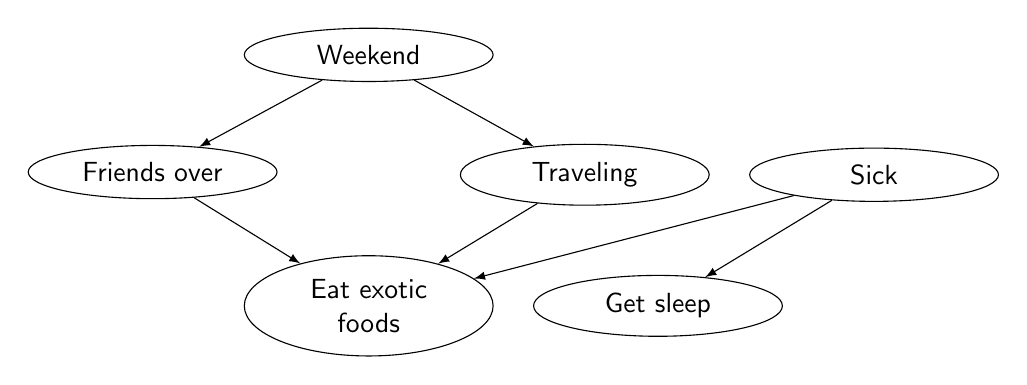
\begin{tikzpicture}[
        node distance=1cm and .5cm,
        bn/.style={draw,ellipse,text width=2cm,align=center}
        ]
        \node[bn] (w) {\attr{Weekend}};
        \node[bn,below right=of w] (t) {\attr{Traveling}};
        \node[bn,right=of t] (s) {\attr{Sick}};
        \node[bn,below left=of w] (f) {\attr{Friends over}};
        \node[bn,below right=of f] (eef) {\attr{Eat exotic foods}};
        \node[bn,right=of eef] (gs) {\attr{Get sleep}};
        \path (w) edge[-latex] (t)
        (w) edge[-latex] (f)
        (f) edge[-latex] (eef)
        (t) edge[-latex] (eef)
        (s) edge[-latex] (gs)
        (s) edge[-latex] (eef);
    \end{tikzpicture}
  \end{center}
  
  \item 
  Yes. If eat exotic foods was observe, than there would be explaining away occurring between friends over and sick such that knowing if friends over would give information on sick. This information would in turn give information on get sleep, so there would be information flow rendering friends over and get sleep not independent.
\end{enumerate}

\newpage
%%%%%%%%%%%%%%%%%%%%%%%%%%%%%%%%%%%%%%%%%%%%%
% Name and Calibration
%%%%%%%%%%%%%%%%%%%%%%%%%%%%%%%%%%%%%%%%%%%%%
\subsection*{Name}
Rodney Lafuente
\subsection*{Collaborators and Resources}
Whom did you work with, and did you use any resources beyond cs181-textbook and your notes?
I did not work with anyone on this problem set.
\subsection*{Calibration}
Approximately how long did this homework take you to complete (in hours)? 
20+
\end{document}
